\documentclass{standalone}

\usepackage{tikz}

\begin{document}
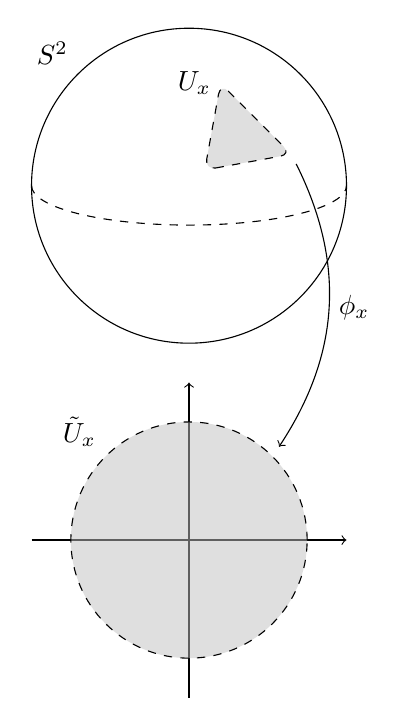
\begin{tikzpicture}
	\draw (0,0) circle[radius=2];
	\draw[dashed] (-2,0) arc[start angle=180, end angle=360, x radius=2, y
			radius=0.5];
	\filldraw[rounded corners, dashed, fill=gray!50, fill opacity=0.5] (0.2, 0.2)
	-- (1.3, 0.4) node(u){} -- (0.4, 1.3) node[left, opacity=1]{$ U_x $} -- cycle;
	\node[above left] at (135:2){$ S^{2} $};

	\begin{scope}[yshift=-4.5cm]
		\draw[->] (-2, 0) -- (2,0);
		\draw[->] (0, -2) -- (0,2);
		\filldraw[dashed, fill=gray!50, fill opacity=0.5] (0,0) circle (1.5);
		\node (v) at (45:1.5){};
		\node[above left] at (135:1.5){$ \tilde{U} _{x} $};
	\end{scope}

	\draw[->, bend left] (u) to node[right]{$ \phi_x $} (v);
\end{tikzpicture}
\end{document}

